\chapter[Herramientas de control y simulación empleadas]{Herramientas de control y simulación empleadas en el trabajo}

A lo largo de este capítulo se efectuará una breve introducción a los distintos aspectos importantes empleados a lo largo del desarrollo del presente trabajo, sin los cuales la comprensión del mismo podría resultar compleja. \par 

Se comenzará efectuando una introducción a distintos aspectos de la teleoperación (una breve evolución histórica, sus elementos constitutivos y distintos sistemas de control en estos entornos). Se continuará con una descripción de distintas herramientas empleadas en el desarrollo de aplicaciones en robótica como pueden ser distintos \emph{Entornos de Desarrollo para Robots}, o \acrshort{rde}s (del inglés, \emph{Robot Development Environment}), o simuladores como \emph{Gazebo}. Posteriormente se realizará una definición de ciertos conceptos relacionados con \emph{modelos en el espacio de estado} (ecuaciones del modelo de estado, observabilidad y observadores del estado) y se finalizará con el cambio en los algoritmos de control que supuso la inclusión de distintos procesos estocásticos en el modelado de sistemas. \par 

\newpage
\section{Introducción a la teleoperación.}

A continuación se mostrará un desarrollo de distintos puntos de la telerrobótica, desde su historia hasta elementos constituyentes de la misma. Para un desarrollo más amplio acerca de la teleoperación y telerrobótica consúltese \cite{barrientos2007fundamentos}. \par 

\subsection{Introducción histórica a la teleoperación.}

Los primeros dispositivos que pueden ser encuadrados dentro de la teleoperación surgieron por la necesidad, a mediados del sigo XX, de manipular elementos radioactivos de manera segura. En estas situaciones el contacto directo entre los materiales manipulados y el operario humano habían de ser evitadas. \par 

Ante esta situación se desarrollaron dispositivos maestro-esclavo, en el que un manipulador esclavo imita los movimientos efectuados por un dispositivo maestro, siendo éste controlado por un operador humano. \par 

En los inicios de la teleoperación, la unión entre maestro y esclavo se efectuaba mecánicamente (un ejemplo de este mecanismo puede apreciarse en la figura \ref{fig:M1-manipulador}), y posteriormente fueron incluyéndose elementos servocotrolados que permitieron una separación física entre maestro y esclavo. \par 

\begin{figure}[h!]
\centering
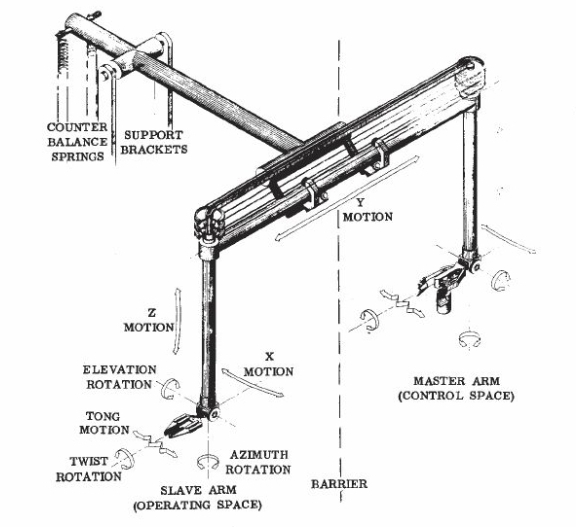
\includegraphics[scale=0.65]{Figuras/M1-manipulador}
\caption[Sistema teleoperado maestro-esclavo M1]{Sistema teleoperado maestro-esclavo M1, desarrollado por \emph{Argonne National Laboratory}. Se trata de uno de los primeros sistemas teleoperados, empleado para manipulación de elementos radioactivos.}
\label{fig:M1-manipulador}
\end{figure}

En estos sistemas servocontrolados suele realizarse un control bilateral, en el que si el maestro realiza una trayectoria, el esclavo la reproduce fielmente y viceversa, o si el esclavo se topa con un obstáculo que le impide el movimiento, este esfuerzo es transmitido al maestro. Este tipo de control pretende simular la unión mecánica existente entre maestro y esclavo de los primeros dispositivos teleoperados creados, en los que el operador era capaz de sentir las fuerzas resultantes de la interacción del esclavo con el entorno. \par 

Esta introducción de dispositivos servocotrolados supuso un gran avance en los sistemas teleoperados debido a la posibilidad de separación física del esclavo y el maestro y así aumentar la distancia existente entre ambos, a la posibilidad de adecuar las fuerzas reflejadas en cada dispositivo y a la gran versatilidad que supone poder modificar el tamaño de los dispositivos maestro y esclavo. Por otro lado, esto supuso un aumento en la complejidad del sistema de control necesario para efectuar el control bilateral, puesto que éste se realiza mediante electrónica analógica en un comienzo, y digital posteriormente y en la actualidad. \par 

A continuación se mostrarán otra serie de principios y elementos propios de la teleoperación, como son los elementos constitutivos de un sistema teleoperado, o los sistemas de control típicamente empleados en estos sistemas. \par 

\subsection{Elementos de un sistema de teleoperación.}

Para que un sistema teleoperado pueda funcionar correctamente, éste debe disponer de una serie de elementos constitutivos principales. El sistema de teleoperación más general, debe constar de los siguientes elementos, según se muestra en \cite{barrientos2007fundamentos}:

\begin{itemize}

\item \emph{Operador humano}: persona encargada de realizar el control a distancia del dispositivo remoto. \par 

\item \emph{Dispositivo teleoperado}: manipulador que realiza las acciones indicadas por el operador humano en el entorno remoto. \par 

\item \emph{Dispositivos de control}: elementos encargados de generar el nexo entre el operador y el entorno remoto. \par 

\item \emph{Dispositivos de realimentación}: elementos encargados de realimentar al operador cierta información del entorno remoto. \par 
 
\item \emph{Control y canales de comunicación}: dispositivos que controlan la comunicación existente entre el entorno local y el remoto. \par 

\item \emph{Sensores}: elementos capaces de medir información necesaria para conocer en cierta medida el entorno remoto y que así puedan ser empleados para realimentación o control. \par 

\end{itemize}

Estos elementos descritos responden al sistema general típico de teleoperación, pudiendo existir otras alternativas con elementos distintos, pero con funcionalidad similar. \par 

\subsection{Control en sistemas teleoperados.}

Una vez descritos los elementos constituyentes de un sistema de teleoperación, es preciso ahora entrar en la descripción de las distintas alternativas de control existentes en estos sistemas. \par 

A lo largo de la historia de la teleoperación se han desarrollado distintos métodos de control para estos sistemas. Todos ellos pueden estar clasificados en dos grupos: \emph{control unilateral} y \emph{control bilateral}. Estos grupos se diferencian en la información que se transmite del entorno local al remoto y viceversa. \par 

\subsubsection{Control unilateral.}

En este tipo de sistemas de control, la información solamente fluye de maestro a esclavo, sin existir realimentación alguna del esclavo al maestro, por esto también recibe el nombre de \emph{control en bucle abierto}. \par 

El manipulador o dispositivo maestro envía instrucciones de posición o velocidad al sistema remoto, y en éste es el sistema de control cinemático el que se encarga de efectuar estos movimientos. \par 

El dispositivo de control maestro, debido a que no se recircula información hacia el maestro no precisa estar actuado, es decir, se trata de un dispositivo pasivo con \emph{encoders} o sensores de posición y/o velocidad. \par 

Debido a su mayor sencillez, es el que fue instalado en los primeros sistemas servocontrolados. \par 

\subsubsection{Control bilateral.}

Por otro lado, en un sistema de \emph{control bilateral} la información fluye en ambos sentidos, desde el maestro hasta el esclavo y al contrario, siendo este tipo más completo que el anterior. \par

La información transmitida desde el maestro hasta el manipulador esclavo, al igual que en el \emph{control unilateral}, consiste generalmente en señales de control de posición y/o velocidad. \par 

La inclusión de una reflexión de fuerzas desde el sistema esclavo al maestro hace que el lazo de control se cierre y exista flujo de información en ambos sentidos. Esta reflexión de fuerzas puede efectuarse de diversas maneras, siendo la reflexión háptica o cinestésica de las mismas la más frecuente, debido a la mayor naturalidad y efectividad que supone el uso del sentido del tacto para una correcta teleoperación. Otras alternativas pueden ser la reflexión visual o sonora de las fuerzas. \par 

Además o en vez de efectuar la reflexión de fuerzas, la información que llega al maestro puede ser de posición y/o velocidad. \par 

En este caso el maestro sí se encuentra motorizado debido a los esfuerzos que debe reflejar al operador, por lo que es un dispositivo activo o actuado. \par 

Dentro del amplio grupo que supone el \emph{control bilateral}, existen distintas alternativas, como se puede apreciar de lo descrito con anterioridad. Estas alternativas se diferencian en el tipo de señales intercambiadas entre el sistema maestro y el esclavo, y son: 

\begin{itemize}

\item \emph{Control bilateral posición-posición}: El control del esclavo se realiza mediante un bucle de posición con referencia de posición y/o velocidad del maestro y al revés, el control del maestro se realiza con un bucle de posición con referencia de posición y/o velocidad del esclavo. Esta variante fue la instaurada en los primeros sistemas de control bilateral. \par 

\item \emph{Control bilateral fuerza-posición}: El control del esclavo se efectúa mediante un bucle de posición con referencia de posición y/o velocidad del maestro, y en cambio, el control del maestro se realiza mediante la realimentación de las fuerzas sentidas por el esclavo. \par 

En este grupo también se incluye aquellos sistemas de control servo de fuerza-posición, en los que se incluye en la realimentación un bucle de control de fuerza del maestro, con la finalidad de anular las componentes de inercia o rozamiento que puedan aparecer en el maestro. \par 

\end{itemize}

\section{Entornos de desarrollo para robots (RDEs).}

El desarrollo de aplicaciones robóticas supone un arduo trabajo de elevada complejidad. En ellas se combinan elementos de diversos ámbitos como puede ser la mecánica, la electrónica, la hidráulica, o ciencia de computadores. \par 

Ante esta heterogénea mezcla de elementos, y con el fin de facilitar el desarrollo de \emph{software} para aplicaciones robóticas surgieron los denominados \acrshort{rde}s (del inglés \emph{Robot Development Environments}). \par 

La gran complejidad y diversidad existente en el desarrollo de aplicaciones robóticas supone una de las grandes dificultades existentes para las mismas. Cada sistema robótico es diferente y distinto al resto, por lo que cada fragmento de \emph{software} tiende a ser específico para cada combinación de \emph{hardware} empleada, debido a la necesidad de interactuar a bajo nivel con los dispositivos y controladores de los mismos. Esta situación hace que la reutilización de \emph{software} entre distintos sistemas y aplicaciones robóticas sea compleja y complicada. Además, esta estrecha relación del \emph{software} y \emph{hardware} hace complicada la separación entre aquellos aspectos a bajo nivel de los de alto nivel. \par 

Estas dificultades y otras consideradas por distintos desarrolladores son las que han levado a la creación de los diversos \acrshort{rde}s desarrollados en la historia, pudiéndose observar una amplia lista de \acrshort{rde}s en \cite{kramer2007development}, afrontando cada uno una serie de dificultades distintas. \par 

Uno de los entornos que más apoyo recibe de distintos desarrolladores y uno de los más activos es \acrshort{ros} (del inglés \emph{Robot Operating System},o \emph{Sistema Operativo para Robots}). Este entorno surge con el objetivo de integrar las distintas soluciones planteadas en la robótica para hacerlo versátil y reutilizable por un amplio grupo de desarrolladores. \par 

A continuación se realizará una breve descripción del entorno \acrshort{ros}, y del simulador robótico \emph{Gazebo}, el cual es empleado también para la prueba y verificación de las distintas aplicaciones desarrolladas en \acrshort{ros}. \par 

\subsection{ROS.}

El \emph{Sistema Operativo para Robots} fue creado en la Universidad de Stanford (E.E.U.U.), en el Laboratorio de Inteligencia Artificial de dicha universidad como parte del proyecto \acrshort{stair} (del inglés \emph{STanford Artificial Intelligence Robot}) para el desarrollo de un robot de servicio con el mismo nombre. \par 

No se trata de un sistema operativo como tal, sino que forma una capa de herramientas, útiles para el desarrollo de aplicaciones robóticas, que se sitúa generalmente sobre un sistema operativo del tipo GNU/Linux, estando más concretamente desarrollado para Ubuntu, aunque puede ser usada, en mayor o menor medida, en otras distribuciones GNU/Linux. \par 

Las bases en las que se creó este entorno pueden consultarse en \cite{quigley2009ros}, y a continuación se muestran resumidos los objetivos bajo los cuales se desarrollo este \emph{framework}, debido a la importancia que supone en la arquitectura final adoptada para \acrshort{ros}:

\begin{itemize}

\item Red \emph{peer-to-peer} (\acrshort{p2p}): estructura descentralizada en la que cada dispositivo de la red funciona como un nodo del mismo nivel que los demás, y atiende y solicita servicios al resto de elementos de la red. Este tipo de red se sitúa en contraposición a la estructura cliente-servidor, en la que es el servidor el que centraliza los procesos y son los clientes los que solicitan servicios al mismo. \par 

\item Multilingüe: Debido a la ambición existente de extender el uso de ROS para el desarrollo de aplicaciones robóticas, \acrshort{ros} fue diseñado para ser compatible con distintos lenguajes de programación, como C++ o Python, y así facilitar su uso a distintos desarrolladores con distintas preferencias. \par 

\item Micronúcleo: El núcleo del entorno se basa en un conjunto heterogéneo de pequeñas herramientas o módulos, cada uno con una funcionalidad específica, para llevar a cabo las actividades necesarias para una aplicación robótica y facilitar su desarrollo. \par 

\item Reutilizable: Para conseguir la reutilización de código, el desarrollo de las aplicaciones se realiza reduciendo las dependencias con las herramientas de \acrshort{ros}, haciendo que éstos sean independientes unos de otros. Situando prácticamente toda la complejidad en las librerías, se pretende conseguir la necesidad de desarrollar únicamente pequeños fragmentos de código para cada aplicación, y que por tanto pueda ser reutilizable para otras. \par 

\item Gratuito y de Código Abierto: \acrshort{ros} es publicado bajo licencia BSD, lo que permite copiar, modificar y redistribuir libremente el código existente en el mismo, lo que facilita la contribución de millones de personas para mejorar este entorno. \par 

\end{itemize}

La implantación de cualquier aplicación basada en \acrshort{ros} precisa el uso de una nomenclatura concreta, que refleja la estructura bajo la cual se organiza un proyecto desarrollado en este entorno:

\begin{itemize}

\item Cada código ejecutable constituye un \emph{nodo}, que presenta una funcionalidad concreta. Son procesos que ejecutan un algoritmo computacional determinado. \par 

\item Los distintos \emph{nodos} se comunican entre sí mediante el uso de \emph{mensajes}, cuya estructura y tipología se encuentra estrictamente definida. Están formados por conjuntos ordenados de los distintos tipos básicos de datos (números enteros, booleanos, cadenas de caracteres, números en coma flotante, etc.). \par 

\item Los \emph{nodos} envían los \emph{mensajes} publicándolos en los denominados \emph{topics}, que conforman la vía de comunicación del \emph{mensaje}. Para recibir la información de estos \emph{mensajes}, los \emph{nodos} deben suscribirse a uno o varios \emph{topics}. Pueden existir múltiples nodos publicando y suscribiéndose al mismo \emph{topic} simultáneamente. \par 

\end{itemize}

Esta estructura refleja la elevada descentralización existente entre los distintos procesos de la red \acrlong{p2p}.

\subsection{\textit{Gazebo}.}

Gazebo es considerado como uno de los simuladores robóticos de código abierto más completos, y éste, en sus orígenes, se encontraba íntimamente ligado a \acrshort{ros}. Al igual que éste, se encuentra estructurado en módulos que forman una red de topología \acrlong{p2p}. \par 

\emph{Gazebo} surge con el objetivo de crear un simulador en 3D multi-robot dinámico de código abierto. Todas las herramientas empleadas para el desarrollo de \emph{Gazebo} son, por tanto, de código abierto, como puede ser el motor físico empleado por defecto denominado \acrshort{ode} (del inglés \emph{Open Dynamics Engine}), o la librería para crear los entornos en 3D openGL, entre otros. \par 

Un desarrollo más extenso de la estructura y arquitectura de Gazebo en sus inicios puede encontrarse en \cite{koenig2004design}, o puede consultarse su dirección web \cite{website:gazebo} para obtener información reciente. A continuación se muestran los elementos principales que constituyen los modelos de robots para ser empleados por Gazebo:

\begin{itemize}

\item Los modelos de robots están formados por distintos elementos denominados \emph{links}, unidos mediante \emph{joints} o uniones. Para cada elemento es preciso determinar una geometría (mediante un modelo \acrshort{cad} del elemento) y una masa e inercia, necesarias para el motor físico, y para las uniones es preciso determinar el tipo de enlace existente entre los distintos elementos, pudiendo ser un par de rotación, cilíndrico, prismático, etc. \par 

\item El conocimiento del entorno se realiza mediante \emph{sensores}, elementos abstractos que carecen de representación física y son los encargados de medir determinadas magnitudes del entorno. Estos \emph{sensores} pretenden imitar el comportamiento real de los mismos, pudiendo incluirse ruido y errores en sus medidas. \par 

\item El movimiento efectuado por el robot se realiza mediante \emph{actuadores}, encargados de interactuar con el motor físico de Gazebo para producir un movimiento determinado, como puede ser aplicar un momento al eje motriz de las ruedas de un robot móvil. \par 

\end{itemize}

Estos \emph{sensores} y \emph{actuadores} pueden ser englobados en los denominados \emph{plugins}, encargados de dotar de funcionalidad las simulaciones de \emph{Gazebo}. 

Para interactuar entre \acrshort{ros} y \emph{Gazebo} existen ciertos paquetes que emplean la \acrshort{api} de \emph{Gazebo} y los denominados \textit{plugins}, lo que permite intercambiar información entre distintos módulos de ambos entornos. Un esquema general de estos paquetes se puede ver en la figura \ref{fig:gazebo-ros}.\par 

\begin{figure}[h!]
\centering
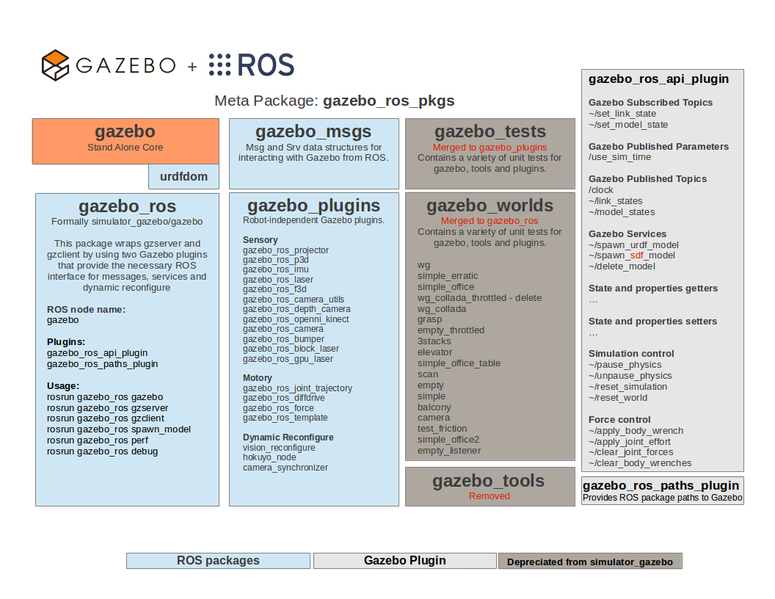
\includegraphics[scale=0.7]{Figuras/Gazebo_ros_api}
\caption[Esquema general de la interacción entre Gazebo y ROS]{Esquema general de la interacción entre Gazebo y ROS. Se muestra el conjunto de paquetes de \emph{software} existente para la interacción del entorno ROS con el simulador \emph{Gazebo}.}
\label{fig:gazebo-ros}
\end{figure}

En el anterior esquema se puede apreciar que alrededor de la aplicación \emph{Gazebo} se han desarrollado una serie de herramientas que permiten el intercambio de información entre las distintas aplicaciones desarrolladas con \acrshort{ros} y \emph{Gazebo}. \par 

Mediante el uso de estas herramientas se puede acceder a la información manejada por el simulador y, de esta manera, poder efectuar una simulación más cercana a la realidad del sistema a verificar y analizar. \par  

\section{Variables de estado.}

Debido a la enorme importancia del estudio de sistemas mediante la formulación en variables de estado en la teoría de control moderna y en las recientes aplicaciones efectuadas a la robótica es preciso mostrar una breve introducción al nuevo paradigma de control que supuso el uso de Variables de Estado con respecto a la teoría de control clásica. Para mayor información puede consultarse \cite{dominguez2000control} o \cite{katsuhiko2010modern}. \par 

El \emph{método del espacio de estado} surgió para el estudio de sistemas dinámicos, el cual busca el conocimiento del comportamiento interno del sistema estudiado, mostrado o reflejado por las denominadas \emph{variables de estado}. Este paradigma busca conocer la máxima información posible del sistema, con el fin de poder controlarlo con mayor precisión. El uso de este modelo de estudio de los sistemas supone un avance para el modelado de sistemas complejos, multivariables y/o no lineales. \par 

Se ha empleado el concepto de \emph{estado de un sistema}, el cual es preciso definir, como se muestra en \cite{dominguez2000control}:

\newtheorem{defin1}{Definición}

\begin{defin1} \textbf{Estado de un sistema}: la mínima cantidad de información necesaria en un instante para que, conociendo la entrada a partir de ese instante, se pueda determinar la salida en cualquier instante posterior.
\end{defin1} 

El estado del sistema viene representado por una serie de variables denominadas variables de estado, que en su conjunto forman el \emph{vector de estado}. Estas variables de estado son las encargadas de representar la situación del sistema en cada instante y para los momentos anteriores, es decir, la \emph{historia} del sistema. \par 

El \emph{vector de estado} constituye una base del espacio vectorial que supone el \emph{espacio de estado}, en el cual el \emph{vector de estado} toma valores. \par 

La representación más común para definir el comportamiento de un sistema dinámico diferencial, incluyendo estados, $\boldsymbol{x}(t)$, entradas, $\boldsymbol{u}(t)$, y salidas, $\boldsymbol{y}(t)$, consta de dos ecuaciones: \emph{ecuación de estado} y \emph{ecuación de salida}. La primera de ellas relaciona la evolución a lo largo del tiempo del estado del sistema, y la segunda relaciona el estado y las entradas con las salidas. Esta representación toma la forma:

\begin{subequations}
\begin{align}
	\boldsymbol{\dot{x}}(t) &= f(t,\boldsymbol{x}(t),\boldsymbol{u}(t)) \\
	\boldsymbol{y}(t) &= h(t,\boldsymbol{x}(t),\boldsymbol{u}(t))
\end{align}
\label{eq:lineal}
\end{subequations}

Estas expresiones son válidas para sistemas físicos, en los que sus variables y estados son continuos. \par 

En contraposición, el extendido empleo del computador para análisis y control de sistemas, lleva a la formulación de las anteriores expresiones para sistemas discretos: 

\begin{subequations}
\begin{align}
	\boldsymbol{x}_{k+1} &= f(k,\boldsymbol{x}_k,\boldsymbol{u}_k) \\
	\boldsymbol{y}_k &= h(k,\boldsymbol{x}_k,\boldsymbol{u}_k)
\end{align}
\end{subequations}

La principal diferencia entre ambas es la aparición de secuencias en todas aquellas variables del sistema, en vez de magnitudes continuas, como sucede en el caso de sistemas continuos. \par 

Puede apreciarse que las expresiones anteriores expresan de forma genérica, mediante unas funciones $f$ y $h$ las relaciones existentes entre las distintas variables. Esta relación puede ser lineal (\emph{sistemas lineales}), siendo éste el caso más estudiado debido a su mayor sencillez, o no lineal (\emph{sistemas no lineales}). \par 

Las distintas ramas de la teoría moderna de control se basan en la representación de la dinámica del sistema en \emph{variables de estado} utilizando cada una unas técnicas distintas. Esta representación ha facilitado el desarrollo de los distintos paradigmas de la teoría de control hacia soluciones más sofisticadas y completas. \par 

Se detallarán seguidamente los conceptos de observabilidad de sistemas y ciertos aspectos de importancia acerca de los denominados observadores del estado.

\subsection{Observabilidad y observadores del estado.}

La observabilidad de un sistema puede entenderse como la posibilidad de conocer la evolución del estado del sistema a partir del conocimiento del valor de las entradas y salidas. Definiciones más rigurosas de observabilidad pueden encontrarse en \cite{dominguez2000control}, las cuales se muestran a continuación:

\newtheorem{defin}{Definición}

\begin{defin} \textbf{Observabilidad}.
Se dice que un punto $\boldsymbol{x}_0$ del espacio de estado es observable en $[t_0,t_1]$ si siendo éste el estado inicial en el instante $t_0$, $\boldsymbol{x}_0 = \boldsymbol{x}(t_0)$, el conocimiento de la entrada $\boldsymbol{u}(t)$ en el intervalo $[t_0,t_1]$ y de la salida $\boldsymbol{y}(t)$ en el mismo intervalo permite determinar que el estado inicial del sistema en el instante $t_0$ es $\boldsymbol{x}_0$.
\end{defin}

\begin{defin} \textbf{Observabilidad para cualquier instante}.
Se dice que un punto $\boldsymbol{x}_0$ del espacio de estado es observable si siendo éste el estado inicial para un instante inicial $t_0$ cualquiera, existe in intervalo de tiempo finito en $[t_0,t_1]$ tal que el conocimiento de la entrada $\boldsymbol{u}(t)$ en el intervalo $[t_0,t_1]$ y de la salida $\boldsymbol{y}(t)$ en el mismo intervalo permite determinar que el estado inicial del sistema es $\boldsymbol{x}_0$.
\end{defin}

\begin{defin} \textbf{Observabilidad de un sistema para un intervalo $[t_0,t_1]$}.
Se dice que un sistema es observable en $[t_0,t_1]$ si todos los puntos del espacio de estado son observables en $[t_0,t_1]$.
\end{defin}

\begin{defin} \textbf{Observabilidad de un sistema}.
Se dice que un sistema es observable si todos los puntos del espacio de estado son observables.
\end{defin}

La observabilidad indica, por tanto, la posibilidad, o no, de poder conocer el estado del sistema en todo momento a partir de la información de las entradas y salidas, por lo que es fundamental su determinación para garantizar el funcionamiento de un \emph{Observador del Estado}. \par 

El Observador del Estado es el encargado de efectuar las estimaciones acerca del estado del sistema $\hat{x}$, a partir de la información entrante y saliente del sistema. Para que un sistema sea observador de un sistema como el definido por las ecuaciones (\ref{eq:lineal}), ha de cumplir una serie de requisitos, tal y como se expresa en \cite{dominguez2000control} y a continuación:

\begin{enumerate}

\item Si los estados de ambos sistemas coinciden en un instante $t_0$, $\hat{x}(t_0) = x(t_0)$, entonces los estados coinciden para todo instante posterior para cualquier entrada $u(t)$ aplicada sobre el sistema. \par 

\item $\hat{x}(t)$ debe tender asintóticamente al estado $x(t)$ para cualquier entrada $u(t)$ y para cualesquiera estados iniciales $\hat{x}(t_0)$ y $x(t_0)$. \par 

\end{enumerate}

Ante estas restricciones, puede deducirse que el sistema observador no puede presentar cualquier morfología ni comportamiento. Existen numerosas alternativas para la formulación de sistemas observadores, y en este texto, se efectuará una implantación de un observador basado en un Filtro de Kalman, explicado en el próximo capítulo. \par 

\section{Procesos estocásticos en sistemas de control.}

Cada vez con mayor asiduidad se busca extender el uso sistemas robóticos o robotizados más allá de entornos industriales, en los que el entorno es en gran medida conocido y estructurado. Esta poca estructuración del entorno origina la necesidad de adaptar aquellos algoritmos de control en los que se requiere un conocimiento exacto del entorno por otros que consideran indeterminaciones en su funcionamiento. \par 

Por este motivo, en las últimas décadas se ha extendido el uso de un enfoque estadístico para hacer frente a estas indeterminaciones inherentes al trabajo en entornos poco estructurados o, al menos, menos estructurados que los existentes en líneas de montaje industriales. \par 

El uso de sensores y actuadores, que en la práctica es imposible que sean completamente exactos, modelos aproximados y entornos desestructurados hace indispensable considerar un cambio en los paradigmas de la robótica: pasar de certezas a probabilidades. \par 

La aplicación de la visión estocástica a la robótica se ha ayudado en gran medida del uso de \emph{modelos del espacio de estado} descritos brevemente con anterioridad, permitiendo igualmente una manera natural de aunar información proveniente de distintas fuentes o sensores (fusión sensorial). \par 

Múltiples aplicaciones han surgido a lo largo de la historia para llevar a cabo este enfoque, como puede ser el \emph{Filtro de Bayes}, el \emph{Filtro de Kalman} o el \emph{Filtro de Partículas}. Una detallada descripción de estos métodos puede encontrarse en \cite{thrun2005probabilistic}. Gran parte de estos métodos basan su funcionamiento en la fusión sensorial, con el fin de poder presentar una descripción más completa y robusta del entorno. Una descripción de distintos métodos de fusión sensorial puede encontrarse en \cite{siciliano2008springer}. \par 

Los distintos métodos mencionados basan su funcionamiento en la denominada \emph{Regla de Bayes}, con la cual se pretende extraer información y relacionar las observaciones efectuadas (medidas de los sensores) con el estado del sistema. \par 

\subsection{Regla de Bayes}

\noindent
Consideraciones previas a realizar:

\begin{itemize}

\item Las medidas de los sensores no son exactas, por lo tanto, lo que se obtiene es una probabilidad de los valores medidos, $y$. \par 

\item El estado del sistema describe la situación actual del sistema, $x$. En la gran mayoría de los casos no puede conocerse directamente, por lo que se suele expresar mediante una distribución de probabilidad. \par 

\item El control del estado se efectúa mediante entradas o acciones, $u$. La evolución suele representarse mediante un \emph{modelo en el espacio de estado}. \par 

\end{itemize}

Siguiendo la notación típicamente empleada para la probabilidad, la relación entre estados $x$ y observaciones $y$, más concretamente, la probabilidad de que los valores de los estados y observaciones sean simultáneamente $x$ e $y$, puede representarse de la forma: 

\[ P(x \cap y) = P(x | y)P(y) = P(y | x)P(x) \]

Esta expresión representa la base de la Regla de Bayes, la cual se expresa despejando la probabilidad de $x$ condicionada por la observación $y$, es decir $P(x | y)$. La Regla de Bayes queda de la forma: 

\begin{equation}
	P(x | y) = \frac{P(y | x)P(x)}{P(y)}
\end{equation} \\
\noindent
la cual expresa cuál es la probabilidad de que el el estado del sistema presente un valor determinado, condicionado por la observación $P(x | y)$, en función de las observaciones realizadas $P(y)$, las estimaciones previas del estado $P(x)$ y la estimación de las observaciones para ese estado $P(y | x)$. \par 

Si se dispone de varias observaciones obtenidas en distintos instantes de tiempo $y_1,y_2 \ldots y_n$, la probabilidad acumulada por todas ellas puede expresarse como:

\[
\begin{split}
	P(y_1,y_2 \ldots y_n |x) &= P(y_1 | x)P(y_2 | x)\ldots P(y_n | x) = \prod_{i=1}^n P(y_i | x) \\
	P(x | Y^n) &= C P(x) \prod_{i=1}^n P(y_i | x)
\end{split}	
\]  \\ 
\noindent
donde C es una matriz de constantes empleada para normalizar los valores obtenidos. \par 

Puesto que en la mayoría de las aplicaciones, las observaciones se efectúan a tiempo real, con el fin de evitar recalcular la expresión completa, puede formularse de forma recursiva:

\begin{equation}
	P(x | Y^k) = \frac{P(y_k | x)P(x | Y^{k-1})}{P(y_k | Y^{k-1})}
\end{equation} 

Esta es la formulación empleada por los distintos métodos desarrollados como pueden ser \emph{Filtro de Bayes}, el \emph{Filtro de Kalman} o el \emph{Filtro de Partículas}. Todos ellos pueden considerarse casos particulares del primero, por ejemplo, el Filtro de Kalman es empleado para sistemas lineales y ruido gaussiano, el cual será descrito en mayor profundidad en próximos capítulos del texto debido a su gran importancia en el trabajo realizado. \par 

\noindent
El algoritmo general empleado por todos estos métodos se basa en unos simples pasos:

\begin{itemize}

\item Predicción del estado próximo en función del estado actual y la acción realizada. \par 

\item Actualización de la estimación producida del estado a partir de las observaciones obtenidas del entorno mediante los sensores. \par 

\end{itemize}

En el próximo capítulo se desarrollará en profundidad el denominado \emph{Filtro de Kalman}, o \acrshort{kf} (del inglés \emph{Kalman FIlter}) y otro algoritmo desarrollado a partir de éste: el \emph{Filtro de Kalman Extendido} o \acrshort{ekf} (del inglés \emph{Extended Kalman Filter}). Se va a mostrar el desarrollo a seguir hasta la formulación de estos dos algoritmos debido a la importancia que presenta en las cualidades y requisitos de estos métodos. \par 